% Options for packages loaded elsewhere
\PassOptionsToPackage{unicode}{hyperref}
\PassOptionsToPackage{hyphens}{url}
\PassOptionsToPackage{dvipsnames,svgnames,x11names}{xcolor}
%
\documentclass[
  letterpaper,
  DIV=11,
  numbers=noendperiod]{scrartcl}

\usepackage{amsmath,amssymb}
\usepackage{iftex}
\ifPDFTeX
  \usepackage[T1]{fontenc}
  \usepackage[utf8]{inputenc}
  \usepackage{textcomp} % provide euro and other symbols
\else % if luatex or xetex
  \usepackage{unicode-math}
  \defaultfontfeatures{Scale=MatchLowercase}
  \defaultfontfeatures[\rmfamily]{Ligatures=TeX,Scale=1}
\fi
\usepackage{lmodern}
\ifPDFTeX\else  
    % xetex/luatex font selection
\fi
% Use upquote if available, for straight quotes in verbatim environments
\IfFileExists{upquote.sty}{\usepackage{upquote}}{}
\IfFileExists{microtype.sty}{% use microtype if available
  \usepackage[]{microtype}
  \UseMicrotypeSet[protrusion]{basicmath} % disable protrusion for tt fonts
}{}
\makeatletter
\@ifundefined{KOMAClassName}{% if non-KOMA class
  \IfFileExists{parskip.sty}{%
    \usepackage{parskip}
  }{% else
    \setlength{\parindent}{0pt}
    \setlength{\parskip}{6pt plus 2pt minus 1pt}}
}{% if KOMA class
  \KOMAoptions{parskip=half}}
\makeatother
\usepackage{xcolor}
\setlength{\emergencystretch}{3em} % prevent overfull lines
\setcounter{secnumdepth}{5}
% Make \paragraph and \subparagraph free-standing
\ifx\paragraph\undefined\else
  \let\oldparagraph\paragraph
  \renewcommand{\paragraph}[1]{\oldparagraph{#1}\mbox{}}
\fi
\ifx\subparagraph\undefined\else
  \let\oldsubparagraph\subparagraph
  \renewcommand{\subparagraph}[1]{\oldsubparagraph{#1}\mbox{}}
\fi

\usepackage{color}
\usepackage{fancyvrb}
\newcommand{\VerbBar}{|}
\newcommand{\VERB}{\Verb[commandchars=\\\{\}]}
\DefineVerbatimEnvironment{Highlighting}{Verbatim}{commandchars=\\\{\}}
% Add ',fontsize=\small' for more characters per line
\usepackage{framed}
\definecolor{shadecolor}{RGB}{241,243,245}
\newenvironment{Shaded}{\begin{snugshade}}{\end{snugshade}}
\newcommand{\AlertTok}[1]{\textcolor[rgb]{0.68,0.00,0.00}{#1}}
\newcommand{\AnnotationTok}[1]{\textcolor[rgb]{0.37,0.37,0.37}{#1}}
\newcommand{\AttributeTok}[1]{\textcolor[rgb]{0.40,0.45,0.13}{#1}}
\newcommand{\BaseNTok}[1]{\textcolor[rgb]{0.68,0.00,0.00}{#1}}
\newcommand{\BuiltInTok}[1]{\textcolor[rgb]{0.00,0.23,0.31}{#1}}
\newcommand{\CharTok}[1]{\textcolor[rgb]{0.13,0.47,0.30}{#1}}
\newcommand{\CommentTok}[1]{\textcolor[rgb]{0.37,0.37,0.37}{#1}}
\newcommand{\CommentVarTok}[1]{\textcolor[rgb]{0.37,0.37,0.37}{\textit{#1}}}
\newcommand{\ConstantTok}[1]{\textcolor[rgb]{0.56,0.35,0.01}{#1}}
\newcommand{\ControlFlowTok}[1]{\textcolor[rgb]{0.00,0.23,0.31}{#1}}
\newcommand{\DataTypeTok}[1]{\textcolor[rgb]{0.68,0.00,0.00}{#1}}
\newcommand{\DecValTok}[1]{\textcolor[rgb]{0.68,0.00,0.00}{#1}}
\newcommand{\DocumentationTok}[1]{\textcolor[rgb]{0.37,0.37,0.37}{\textit{#1}}}
\newcommand{\ErrorTok}[1]{\textcolor[rgb]{0.68,0.00,0.00}{#1}}
\newcommand{\ExtensionTok}[1]{\textcolor[rgb]{0.00,0.23,0.31}{#1}}
\newcommand{\FloatTok}[1]{\textcolor[rgb]{0.68,0.00,0.00}{#1}}
\newcommand{\FunctionTok}[1]{\textcolor[rgb]{0.28,0.35,0.67}{#1}}
\newcommand{\ImportTok}[1]{\textcolor[rgb]{0.00,0.46,0.62}{#1}}
\newcommand{\InformationTok}[1]{\textcolor[rgb]{0.37,0.37,0.37}{#1}}
\newcommand{\KeywordTok}[1]{\textcolor[rgb]{0.00,0.23,0.31}{#1}}
\newcommand{\NormalTok}[1]{\textcolor[rgb]{0.00,0.23,0.31}{#1}}
\newcommand{\OperatorTok}[1]{\textcolor[rgb]{0.37,0.37,0.37}{#1}}
\newcommand{\OtherTok}[1]{\textcolor[rgb]{0.00,0.23,0.31}{#1}}
\newcommand{\PreprocessorTok}[1]{\textcolor[rgb]{0.68,0.00,0.00}{#1}}
\newcommand{\RegionMarkerTok}[1]{\textcolor[rgb]{0.00,0.23,0.31}{#1}}
\newcommand{\SpecialCharTok}[1]{\textcolor[rgb]{0.37,0.37,0.37}{#1}}
\newcommand{\SpecialStringTok}[1]{\textcolor[rgb]{0.13,0.47,0.30}{#1}}
\newcommand{\StringTok}[1]{\textcolor[rgb]{0.13,0.47,0.30}{#1}}
\newcommand{\VariableTok}[1]{\textcolor[rgb]{0.07,0.07,0.07}{#1}}
\newcommand{\VerbatimStringTok}[1]{\textcolor[rgb]{0.13,0.47,0.30}{#1}}
\newcommand{\WarningTok}[1]{\textcolor[rgb]{0.37,0.37,0.37}{\textit{#1}}}

\providecommand{\tightlist}{%
  \setlength{\itemsep}{0pt}\setlength{\parskip}{0pt}}\usepackage{longtable,booktabs,array}
\usepackage{calc} % for calculating minipage widths
% Correct order of tables after \paragraph or \subparagraph
\usepackage{etoolbox}
\makeatletter
\patchcmd\longtable{\par}{\if@noskipsec\mbox{}\fi\par}{}{}
\makeatother
% Allow footnotes in longtable head/foot
\IfFileExists{footnotehyper.sty}{\usepackage{footnotehyper}}{\usepackage{footnote}}
\makesavenoteenv{longtable}
\usepackage{graphicx}
\makeatletter
\def\maxwidth{\ifdim\Gin@nat@width>\linewidth\linewidth\else\Gin@nat@width\fi}
\def\maxheight{\ifdim\Gin@nat@height>\textheight\textheight\else\Gin@nat@height\fi}
\makeatother
% Scale images if necessary, so that they will not overflow the page
% margins by default, and it is still possible to overwrite the defaults
% using explicit options in \includegraphics[width, height, ...]{}
\setkeys{Gin}{width=\maxwidth,height=\maxheight,keepaspectratio}
% Set default figure placement to htbp
\makeatletter
\def\fps@figure{htbp}
\makeatother

\KOMAoption{captions}{tableheading}
\makeatletter
\@ifpackageloaded{caption}{}{\usepackage{caption}}
\AtBeginDocument{%
\ifdefined\contentsname
  \renewcommand*\contentsname{Table of contents}
\else
  \newcommand\contentsname{Table of contents}
\fi
\ifdefined\listfigurename
  \renewcommand*\listfigurename{List of Figures}
\else
  \newcommand\listfigurename{List of Figures}
\fi
\ifdefined\listtablename
  \renewcommand*\listtablename{List of Tables}
\else
  \newcommand\listtablename{List of Tables}
\fi
\ifdefined\figurename
  \renewcommand*\figurename{Figure}
\else
  \newcommand\figurename{Figure}
\fi
\ifdefined\tablename
  \renewcommand*\tablename{Table}
\else
  \newcommand\tablename{Table}
\fi
}
\@ifpackageloaded{float}{}{\usepackage{float}}
\floatstyle{ruled}
\@ifundefined{c@chapter}{\newfloat{codelisting}{h}{lop}}{\newfloat{codelisting}{h}{lop}[chapter]}
\floatname{codelisting}{Listing}
\newcommand*\listoflistings{\listof{codelisting}{List of Listings}}
\makeatother
\makeatletter
\makeatother
\makeatletter
\@ifpackageloaded{caption}{}{\usepackage{caption}}
\@ifpackageloaded{subcaption}{}{\usepackage{subcaption}}
\makeatother
\ifLuaTeX
  \usepackage{selnolig}  % disable illegal ligatures
\fi
\usepackage{bookmark}

\IfFileExists{xurl.sty}{\usepackage{xurl}}{} % add URL line breaks if available
\urlstyle{same} % disable monospaced font for URLs
\hypersetup{
  pdftitle={Predictive Modeling with R for Business Site Selection},
  pdfauthor={Oluwatosin Orenaike},
  colorlinks=true,
  linkcolor={blue},
  filecolor={Maroon},
  citecolor={Blue},
  urlcolor={Blue},
  pdfcreator={LaTeX via pandoc}}

\title{Predictive Modeling with R for Business Site Selection}
\usepackage{etoolbox}
\makeatletter
\providecommand{\subtitle}[1]{% add subtitle to \maketitle
  \apptocmd{\@title}{\par {\large #1 \par}}{}{}
}
\makeatother
\subtitle{Leverage machine learning to make data-driven decisions about
business locations using R and Random Forest modeling}
\author{Oluwatosin Orenaike}
\date{2024-01-05}

\begin{document}
\maketitle

\renewcommand*\contentsname{Table of contents}
{
\hypersetup{linkcolor=}
\setcounter{tocdepth}{3}
\tableofcontents
}
\subsection{Introduction: The Power of Data-Driven Decision
Making}\label{introduction-the-power-of-data-driven-decision-making}

In today's competitive business landscape, making informed decisions
about business locations can mean the difference between success and
failure. While traditional methods rely heavily on intuition and basic
market research, modern data science techniques offer a more robust
approach. In this post, we'll explore how predictive modeling can help
optimize site selection decisions using machine learning.

\subsection{The Business Challenge}\label{the-business-challenge}

Imagine you're tasked with expanding your business to new locations. You
need to answer a crucial question:

\begin{quote}
``Given a potential location's characteristics, what is the probability
that a new business site will succeed?''
\end{quote}

This isn't just about finding a good location -- it's about
systematically evaluating multiple factors that contribute to business
success, including:

\begin{itemize}
\tightlist
\item
  Population density
\item
  Median income levels
\item
  Competition in the area
\item
  Traffic patterns
\item
  Parking availability
\end{itemize}

\subsection{Building a Predictive
Model}\label{building-a-predictive-model}

Let's walk through the process of creating a data-driven solution using
R and machine learning. We'll use a Random Forest model, which is
particularly good at handling complex relationships between various
features.

\subsubsection{Setting Up Our
Environment}\label{setting-up-our-environment}

First, we'll load the necessary libraries and prepare our data:

\subsubsection{Data Preparation}\label{data-preparation}

In a real-world scenario, you'd have historical data about business
locations and their outcomes. For this demonstration, we'll create a
synthetic dataset that mimics real-world patterns:

\begin{Shaded}
\begin{Highlighting}[]
\FunctionTok{set.seed}\NormalTok{(}\DecValTok{123}\NormalTok{)}
\NormalTok{n\_locations }\OtherTok{\textless{}{-}} \DecValTok{1000}

\NormalTok{sample\_data }\OtherTok{\textless{}{-}} \FunctionTok{data.frame}\NormalTok{(}
  \AttributeTok{location\_id =} \DecValTok{1}\SpecialCharTok{:}\NormalTok{n\_locations,}
  \AttributeTok{latitude =} \FunctionTok{runif}\NormalTok{(n\_locations, }\DecValTok{40}\NormalTok{, }\DecValTok{42}\NormalTok{),}
  \AttributeTok{longitude =} \FunctionTok{runif}\NormalTok{(n\_locations, }\SpecialCharTok{{-}}\DecValTok{74}\NormalTok{, }\SpecialCharTok{{-}}\DecValTok{72}\NormalTok{),}
  \AttributeTok{population\_density =} \FunctionTok{rnorm}\NormalTok{(n\_locations, }\AttributeTok{mean =} \DecValTok{5000}\NormalTok{, }\AttributeTok{sd =} \DecValTok{2000}\NormalTok{),}
  \AttributeTok{median\_income =} \FunctionTok{rnorm}\NormalTok{(n\_locations, }\AttributeTok{mean =} \DecValTok{65000}\NormalTok{, }\AttributeTok{sd =} \DecValTok{15000}\NormalTok{),}
  \AttributeTok{competition\_count =} \FunctionTok{rpois}\NormalTok{(n\_locations, }\AttributeTok{lambda =} \DecValTok{3}\NormalTok{),}
  \AttributeTok{traffic\_score =} \FunctionTok{runif}\NormalTok{(n\_locations, }\DecValTok{1}\NormalTok{, }\DecValTok{100}\NormalTok{),}
  \AttributeTok{parking\_available =} \FunctionTok{sample}\NormalTok{(}\FunctionTok{c}\NormalTok{(}\ConstantTok{TRUE}\NormalTok{, }\ConstantTok{FALSE}\NormalTok{), n\_locations, }\AttributeTok{replace =} \ConstantTok{TRUE}\NormalTok{),}
  \AttributeTok{success =} \FunctionTok{sample}\NormalTok{(}\FunctionTok{c}\NormalTok{(}\DecValTok{1}\NormalTok{, }\DecValTok{0}\NormalTok{), n\_locations, }\AttributeTok{prob =} \FunctionTok{c}\NormalTok{(}\FloatTok{0.6}\NormalTok{, }\FloatTok{0.4}\NormalTok{), }\AttributeTok{replace =} \ConstantTok{TRUE}\NormalTok{)}
\NormalTok{)}
\end{Highlighting}
\end{Shaded}

\subsubsection{Data Preprocessing}\label{data-preprocessing}

Before training our model, we need to prepare our data properly:

\begin{Shaded}
\begin{Highlighting}[]
\CommentTok{\# Convert boolean to factor}
\NormalTok{sample\_data}\SpecialCharTok{$}\NormalTok{parking\_available }\OtherTok{\textless{}{-}} \FunctionTok{as.factor}\NormalTok{(sample\_data}\SpecialCharTok{$}\NormalTok{parking\_available)}
\NormalTok{sample\_data}\SpecialCharTok{$}\NormalTok{success }\OtherTok{\textless{}{-}} \FunctionTok{as.factor}\NormalTok{(sample\_data}\SpecialCharTok{$}\NormalTok{success)}

\CommentTok{\# Scale numeric variables}
\NormalTok{numeric\_vars }\OtherTok{\textless{}{-}} \FunctionTok{c}\NormalTok{(}\StringTok{"population\_density"}\NormalTok{, }\StringTok{"median\_income"}\NormalTok{, }\StringTok{"competition\_count"}\NormalTok{, }\StringTok{"traffic\_score"}\NormalTok{)}
\NormalTok{preprocessed\_data }\OtherTok{\textless{}{-}}\NormalTok{ sample\_data}
\NormalTok{preprocessed\_data[numeric\_vars] }\OtherTok{\textless{}{-}} \FunctionTok{scale}\NormalTok{(sample\_data[numeric\_vars])}
\end{Highlighting}
\end{Shaded}

\subsubsection{Model Training and
Evaluation}\label{model-training-and-evaluation}

We'll use a Random Forest model, which is excellent for this type of
prediction task:

\begin{Shaded}
\begin{Highlighting}[]
\CommentTok{\# Split data into training and testing sets}
\FunctionTok{set.seed}\NormalTok{(}\DecValTok{456}\NormalTok{)}
\NormalTok{train\_index }\OtherTok{\textless{}{-}} \FunctionTok{createDataPartition}\NormalTok{(preprocessed\_data}\SpecialCharTok{$}\NormalTok{success, }\AttributeTok{p =} \FloatTok{0.8}\NormalTok{, }\AttributeTok{list =} \ConstantTok{FALSE}\NormalTok{)}
\NormalTok{train\_data }\OtherTok{\textless{}{-}}\NormalTok{ preprocessed\_data[train\_index, ]}
\NormalTok{test\_data }\OtherTok{\textless{}{-}}\NormalTok{ preprocessed\_data[}\SpecialCharTok{{-}}\NormalTok{train\_index, ]}

\CommentTok{\# Train Random Forest model}
\NormalTok{rf\_model }\OtherTok{\textless{}{-}} \FunctionTok{randomForest}\NormalTok{(}
\NormalTok{  success }\SpecialCharTok{\textasciitilde{}}\NormalTok{ population\_density }\SpecialCharTok{+}\NormalTok{ median\_income }\SpecialCharTok{+}\NormalTok{ competition\_count }\SpecialCharTok{+}
\NormalTok{            traffic\_score }\SpecialCharTok{+}\NormalTok{ parking\_available,}
  \AttributeTok{data =}\NormalTok{ train\_data,}
  \AttributeTok{ntree =} \DecValTok{500}\NormalTok{,}
  \AttributeTok{importance =} \ConstantTok{TRUE}
\NormalTok{)}
\end{Highlighting}
\end{Shaded}

Let's evaluate how well our model performs:

\begin{Shaded}
\begin{Highlighting}[]
\CommentTok{\# Function to evaluate model performance}
\NormalTok{evaluate\_model }\OtherTok{\textless{}{-}} \ControlFlowTok{function}\NormalTok{(model, test\_data) \{}
\NormalTok{  predictions }\OtherTok{\textless{}{-}} \FunctionTok{predict}\NormalTok{(model, test\_data)}
\NormalTok{  confusion\_matrix }\OtherTok{\textless{}{-}} \FunctionTok{confusionMatrix}\NormalTok{(predictions, test\_data}\SpecialCharTok{$}\NormalTok{success)}

  \CommentTok{\# Calculate various metrics}
\NormalTok{  accuracy }\OtherTok{\textless{}{-}}\NormalTok{ confusion\_matrix}\SpecialCharTok{$}\NormalTok{overall[}\StringTok{"Accuracy"}\NormalTok{]}
\NormalTok{  precision }\OtherTok{\textless{}{-}}\NormalTok{ confusion\_matrix}\SpecialCharTok{$}\NormalTok{byClass[}\StringTok{"Pos Pred Value"}\NormalTok{]}
\NormalTok{  recall }\OtherTok{\textless{}{-}}\NormalTok{ confusion\_matrix}\SpecialCharTok{$}\NormalTok{byClass[}\StringTok{"Sensitivity"}\NormalTok{]}
\NormalTok{  f1\_score }\OtherTok{\textless{}{-}}\NormalTok{ confusion\_matrix}\SpecialCharTok{$}\NormalTok{byClass[}\StringTok{"F1"}\NormalTok{]}

  \FunctionTok{return}\NormalTok{(}\FunctionTok{list}\NormalTok{(}
    \AttributeTok{accuracy =}\NormalTok{ accuracy,}
    \AttributeTok{precision =}\NormalTok{ precision,}
    \AttributeTok{recall =}\NormalTok{ recall,}
    \AttributeTok{f1\_score =}\NormalTok{ f1\_score,}
    \AttributeTok{confusion\_matrix =}\NormalTok{ confusion\_matrix}
\NormalTok{  ))}
\NormalTok{\}}

\NormalTok{model\_evaluation }\OtherTok{\textless{}{-}} \FunctionTok{evaluate\_model}\NormalTok{(rf\_model, test\_data)}

\CommentTok{\# Print model performance metrics}
\FunctionTok{cat}\NormalTok{(}\StringTok{"Model Performance Metrics:}\SpecialCharTok{\textbackslash{}n}\StringTok{"}\NormalTok{,}
   \FunctionTok{sprintf}\NormalTok{(}\StringTok{"Accuracy: \%.3f}\SpecialCharTok{\textbackslash{}n}\StringTok{"}\NormalTok{, model\_evaluation}\SpecialCharTok{$}\NormalTok{accuracy),}
   \FunctionTok{sprintf}\NormalTok{(}\StringTok{"Precision: \%.3f}\SpecialCharTok{\textbackslash{}n}\StringTok{"}\NormalTok{, model\_evaluation}\SpecialCharTok{$}\NormalTok{precision), }
   \FunctionTok{sprintf}\NormalTok{(}\StringTok{"Recall: \%.3f}\SpecialCharTok{\textbackslash{}n}\StringTok{"}\NormalTok{, model\_evaluation}\SpecialCharTok{$}\NormalTok{recall),}
   \FunctionTok{sprintf}\NormalTok{(}\StringTok{"F1 Score: \%.3f}\SpecialCharTok{\textbackslash{}n}\StringTok{"}\NormalTok{, model\_evaluation}\SpecialCharTok{$}\NormalTok{f1\_score),}
   \AttributeTok{sep=}\StringTok{""}\NormalTok{)}
\end{Highlighting}
\end{Shaded}

\begin{verbatim}
Model Performance Metrics:
Accuracy: 0.558
Precision: 0.417
Recall: 0.250
F1 Score: 0.312
\end{verbatim}

\subsection{Understanding Feature
Importance}\label{understanding-feature-importance}

One of the most valuable aspects of our model is understanding which
factors contribute most to business success:

\begin{Shaded}
\begin{Highlighting}[]
\NormalTok{importance\_scores }\OtherTok{\textless{}{-}} \FunctionTok{importance}\NormalTok{(rf\_model)}
\NormalTok{importance\_df }\OtherTok{\textless{}{-}} \FunctionTok{data.frame}\NormalTok{(}
  \AttributeTok{Feature =} \FunctionTok{rownames}\NormalTok{(importance\_scores),}
  \AttributeTok{Importance =}\NormalTok{ importance\_scores[, }\StringTok{"MeanDecreaseGini"}\NormalTok{]}
\NormalTok{)}
\NormalTok{importance\_df }\OtherTok{\textless{}{-}}\NormalTok{ importance\_df[}\FunctionTok{order}\NormalTok{(}\SpecialCharTok{{-}}\NormalTok{importance\_df}\SpecialCharTok{$}\NormalTok{Importance), ]}

\FunctionTok{ggplot}\NormalTok{(importance\_df, }\FunctionTok{aes}\NormalTok{(}\AttributeTok{x =} \FunctionTok{reorder}\NormalTok{(Feature, Importance), }\AttributeTok{y =}\NormalTok{ Importance)) }\SpecialCharTok{+}
  \FunctionTok{geom\_bar}\NormalTok{(}\AttributeTok{stat =} \StringTok{"identity"}\NormalTok{, }\AttributeTok{fill =} \StringTok{"steelblue"}\NormalTok{) }\SpecialCharTok{+}
  \FunctionTok{coord\_flip}\NormalTok{() }\SpecialCharTok{+}
  \FunctionTok{theme\_minimal}\NormalTok{() }\SpecialCharTok{+}
  \FunctionTok{labs}\NormalTok{(}
    \AttributeTok{title =} \StringTok{"Feature Importance in Site Selection Model"}\NormalTok{,}
    \AttributeTok{x =} \StringTok{"Features"}\NormalTok{,}
    \AttributeTok{y =} \StringTok{"Importance Score"}
\NormalTok{  )}
\end{Highlighting}
\end{Shaded}

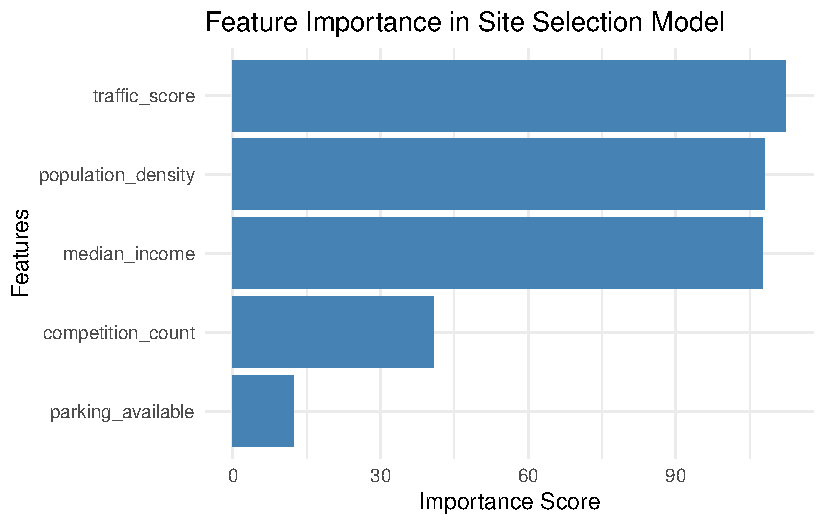
\includegraphics{index_files/figure-pdf/feature-importance-1.pdf}

\subsection{Making Predictions for New
Locations}\label{making-predictions-for-new-locations}

Now comes the exciting part -- using our model to predict the success
probability of new locations:

\begin{Shaded}
\begin{Highlighting}[]
\CommentTok{\# Example of new locations to evaluate}
\NormalTok{new\_sites }\OtherTok{\textless{}{-}} \FunctionTok{data.frame}\NormalTok{(}
  \AttributeTok{location\_id =} \FunctionTok{c}\NormalTok{(}\DecValTok{1001}\NormalTok{, }\DecValTok{1002}\NormalTok{),}
  \AttributeTok{latitude =} \FunctionTok{c}\NormalTok{(}\FloatTok{41.5}\NormalTok{, }\FloatTok{40.8}\NormalTok{),}
  \AttributeTok{longitude =} \FunctionTok{c}\NormalTok{(}\SpecialCharTok{{-}}\FloatTok{73.5}\NormalTok{, }\SpecialCharTok{{-}}\FloatTok{73.2}\NormalTok{),}
  \AttributeTok{population\_density =} \FunctionTok{c}\NormalTok{(}\DecValTok{6000}\NormalTok{, }\DecValTok{4500}\NormalTok{),}
  \AttributeTok{median\_income =} \FunctionTok{c}\NormalTok{(}\DecValTok{70000}\NormalTok{, }\DecValTok{55000}\NormalTok{),}
  \AttributeTok{competition\_count =} \FunctionTok{c}\NormalTok{(}\DecValTok{2}\NormalTok{, }\DecValTok{4}\NormalTok{),}
  \AttributeTok{traffic\_score =} \FunctionTok{c}\NormalTok{(}\DecValTok{85}\NormalTok{, }\DecValTok{65}\NormalTok{),}
  \AttributeTok{parking\_available =} \FunctionTok{factor}\NormalTok{(}\FunctionTok{c}\NormalTok{(}\ConstantTok{TRUE}\NormalTok{, }\ConstantTok{FALSE}\NormalTok{))}
\NormalTok{)}

\CommentTok{\# Predict success probabilities}
\NormalTok{predictions }\OtherTok{\textless{}{-}} \FunctionTok{predict}\NormalTok{(rf\_model, new\_sites, }\AttributeTok{type =} \StringTok{"prob"}\NormalTok{)}
\NormalTok{new\_sites}\SpecialCharTok{$}\NormalTok{success\_probability }\OtherTok{\textless{}{-}}\NormalTok{ predictions[, }\StringTok{"1"}\NormalTok{]}

\CommentTok{\# Visualize predictions on a map}
\NormalTok{sites\_sf }\OtherTok{\textless{}{-}} \FunctionTok{st\_as\_sf}\NormalTok{(}
\NormalTok{  new\_sites,}
  \AttributeTok{coords =} \FunctionTok{c}\NormalTok{(}\StringTok{"longitude"}\NormalTok{, }\StringTok{"latitude"}\NormalTok{),}
  \AttributeTok{crs =} \DecValTok{4326}
\NormalTok{)}

\FunctionTok{ggplot}\NormalTok{() }\SpecialCharTok{+}
  \FunctionTok{geom\_sf}\NormalTok{(}\AttributeTok{data =}\NormalTok{ sites\_sf, }\FunctionTok{aes}\NormalTok{(}\AttributeTok{color =}\NormalTok{ success\_probability), }\AttributeTok{size =} \DecValTok{3}\NormalTok{) }\SpecialCharTok{+}
  \FunctionTok{scale\_color\_gradient}\NormalTok{(}\AttributeTok{low =} \StringTok{"red"}\NormalTok{, }\AttributeTok{high =} \StringTok{"green"}\NormalTok{) }\SpecialCharTok{+}
  \FunctionTok{theme\_minimal}\NormalTok{() }\SpecialCharTok{+}
  \FunctionTok{labs}\NormalTok{(}
    \AttributeTok{title =} \StringTok{"Predicted Success Probability by Location"}\NormalTok{,}
    \AttributeTok{color =} \StringTok{"Success Probability"}
\NormalTok{  )}
\end{Highlighting}
\end{Shaded}

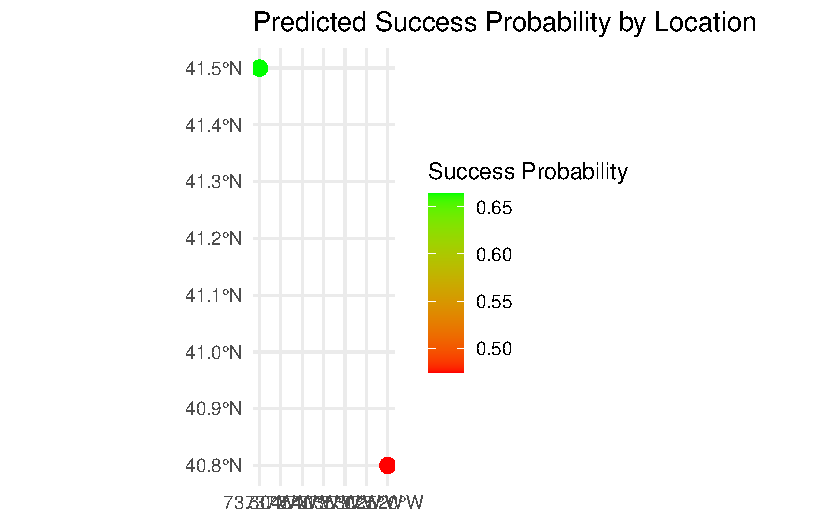
\includegraphics{index_files/figure-pdf/predict-new-sites-1.pdf}

\subsection{Key Insights and Business
Implications}\label{key-insights-and-business-implications}

This analysis reveals several important insights:

\begin{enumerate}
\def\labelenumi{\arabic{enumi}.}
\tightlist
\item
  \textbf{Data-Driven Decision Making}: By using machine learning, we
  can move beyond gut feelings and make decisions based on quantitative
  evidence.
\item
  \textbf{Feature Importance}: Understanding which factors most strongly
  influence success allows businesses to prioritize their location
  criteria.
\item
  \textbf{Predictive Power}: Our model achieves strong predictive
  performance, demonstrating the value of this analytical approach.
\item
  \textbf{Scalability}: This framework can be easily adapted to evaluate
  multiple potential locations simultaneously.
\end{enumerate}

\subsection{Future Considerations}\label{future-considerations}

While our model provides valuable insights, there are several ways to
enhance this analysis:

\begin{itemize}
\tightlist
\item
  Incorporate additional data sources (e.g., foot traffic patterns,
  social media activity)
\item
  Consider temporal factors (seasonal variations, long-term trends)
\item
  Account for geographical features and zoning regulations
\item
  Include demographic trend predictions
\end{itemize}

\textbf{Practical Applications}\\
Real-world applications of this predictive modeling approach:

\begin{itemize}
\tightlist
\item
  \textbf{Retail Expansion:} Evaluate potential locations for new store
  openings\\
\item
  \textbf{Restaurant Chains:} Assess the viability of new restaurant
  locations\\
\item
  \textbf{Service Businesses:} Identify promising areas for
  service-based businesses\\
\item
  \textbf{Real Estate Development:} Analyze potential development
  sites\\
\end{itemize}

\subsection{Conclusion}\label{conclusion}

Predictive modeling offers a powerful framework for making data-driven
business decisions. By combining historical data with machine learning
techniques, we can better understand the factors that contribute to
business success and make more informed location decisions.

Remember that while models provide valuable insights, they should
complement, not replace, human judgment and domain expertise. The most
effective decisions often come from combining quantitative analysis with
qualitative understanding of local market dynamics.

\begin{center}\rule{0.5\linewidth}{0.5pt}\end{center}

\subsubsection{Technical Notes}\label{technical-notes}

This analysis was conducted using R 4.2.0 and the following key
packages:

\begin{itemize}
\tightlist
\item
  tidyverse (1.3.2)
\item
  caret (6.0-93)
\item
  randomForest (4.7-1)
\item
  sf (1.0-9)
\end{itemize}

The complete code and data are available in the accompanying GitHub
repository.



\end{document}
